\documentclass{beamer}
\usepackage[utf8]{inputenc}  % allow utf-8 input
\usepackage[T1]{fontenc}     % use 8-bit T1 fonts
\usepackage{babel,textcomp}
\usepackage[labelformat=empty]{caption}
\usepackage[absolute,overlay]{textpos}
\usepackage{graphicx}
\usepackage{epstopdf}
\usepackage[orientation=landscape,
size=custom,
width=16,
height=9,
scale=0.5]{beamerposter}
% Custom bullets
\usepackage{pifont}
\usepackage{colortbl}
% For showing code in frames
\usepackage{minted}
% \usepackage{shellesc}
% define new colors
\definecolor{LightGray}{RGB}{252,160,140}
\definecolor{LightBlue}{RGB}{176,196,222}

\usetheme{Szeged}
\usecolortheme{crane}


% turn off navigation symbols
\setbeamertemplate{navigation symbols}{}

% Turn on frame numbers
% frame number right-aligned
% \setbeamertemplate{footline}[frame number]
% frame number left-aligned
\setbeamertemplate{footline}{~\insertframenumber{}/\inserttotalframenumber{}\vspace{1mm}}
\setbeamertemplate{headline}{}

% Shadow mode of blocks
\setbeamertemplate{blocks}[rounded][shadow=true]
% 1- Block title (background and text)
\setbeamercolor{block title}{bg=white, fg=black}
% 2- Block body (background)
\setbeamercolor{block body}{bg=lightgray!25}

\title{\textbf{Mininet\\An Instant Virtual Network on your Laptop}}

\author{\textbf{Kristjon Ciko}}
\institute{University of Oslo}

% \vspace{2cm}
\date{\small{Mininet Workshop\newline{}sponsored by\newline{}
    Norwegian Defence Research Establishment (FFI)\newline{}
    \newline{} April 30, 2024}}

\begin{document}

\begin{frame}[plain]
  \titlepage{}
  \addtocounter{framenumber}{-1}
\end{frame}
%------------------------------------------------------------------------------%
\begin{frame}[plain]
  \frametitle{
    \centerline{Mininet:\@ An Instant Virtual Network on your Laptop}}

  \begin{textblock*}{5cm} (1.25cm, 4.2cm) % {block width} (coords)
    \small
    Kristjon Ciko, Ph.D.\newline
    Department of Informatics\newline
    University of Oslo\newline
  \end{textblock*}

  \begin{textblock*}{7.9cm} (6.5cm,4cm) % {block width} (coords)
    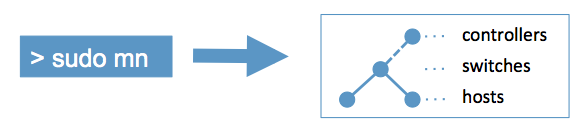
\includegraphics[width=7.9cm]{images/mininet.png}
    \captionsetup[figure]{justification=centering,font=footnotesize}
    \captionof{figure}{[Photo: https://mininet.org]}
  \end{textblock*}

  \begin{textblock*}{4cm} (1.16cm,6.75cm) % {block width} (coords)
    
\includegraphics[width=4cm]{images/uio-ifi.png}
  \end{textblock*}

  \begin{textblock*}{4cm} (1.16cm,7.75cm) % {block width} (coords)
    
\includegraphics[width=4cm]{images/ffi.png}
  \end{textblock*}

  \addtocounter{framenumber}{-1}
\end{frame}
%------------------------------------------------------------------------------%
\begin{frame}
  \frametitle{Who's in this room?!}
\end{frame}

%------------------------------------------------------------------------------%
\begin{frame}
  \frametitle{Who's in this room?!}
  \begin{figure}
    % \vspace{1cm}
    \begin{center}
      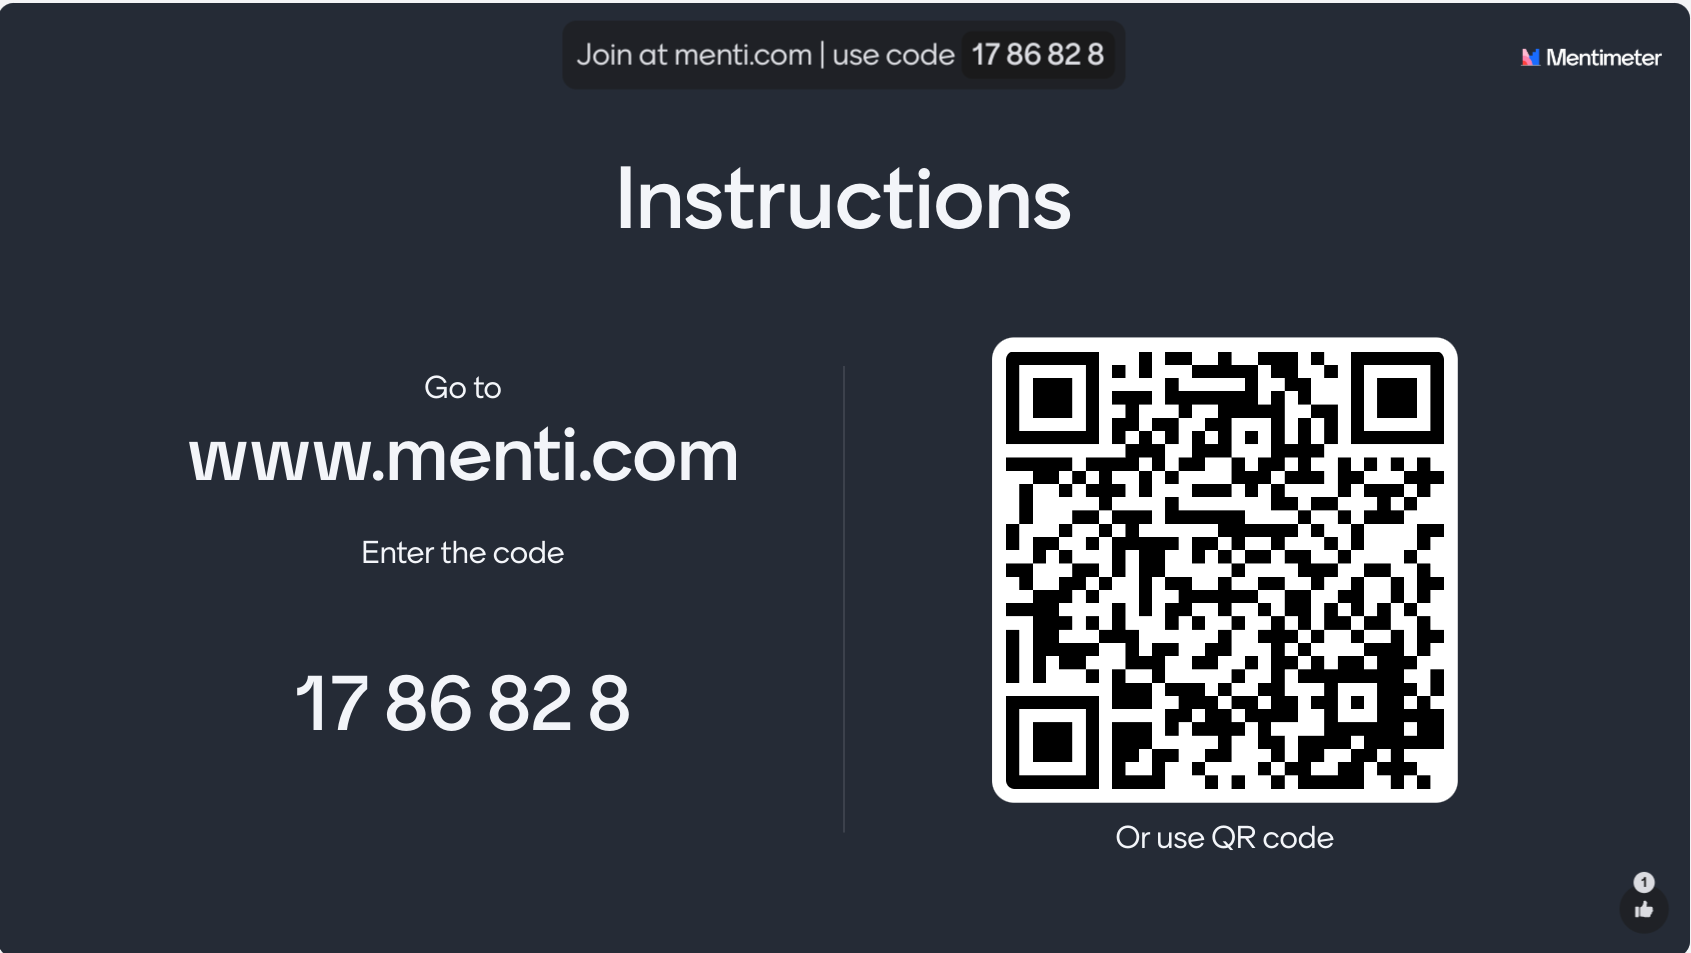
\includegraphics[scale=0.175]{images/menti.png}
    \end{center}
  \end{figure}
\end{frame}

%------------------------------------------------------------------------------%
\begin{frame}
  \frametitle{Goals}
\end{frame}

%------------------------------------------------------------------------------%
%------------------------------------------------------------------------------%
\begin{frame}
  \frametitle{Goals}

  \begin{block}{\textbf{Overarching Goal}} 
    Get familiar with Mininet's core functionalities
  \end{block}

\end{frame}

%------------------------------------------------------------------------------%
%------------------------------------------------------------------------------%
\begin{frame}
  \frametitle{Goals}

  \begin{block}{\textbf{By the end, everyone should know:}}

    \begin{itemize}[<+->]\color{black}
    \item[\ding{51}] \color<.>{black}What is Mininet
    \item[\ding{51}] \color<.>{black} Mininet Command Line Interface (CLI)
    \item[\ding{51}] \color<.>{black}Mininet Python API
    \item[\ding{51}] \color<.>{black} Mininet and Software-Defined
      Networking (SDN)
    \end{itemize}

  \end{block}

\end{frame}

%------------------------------------------------------------------------------%
%------------------------------------------------------------------------------%
\begin{frame}
  \frametitle{Agenda}

  \centering
  \begin{tabular}{cc}
    \hline
    \rowcolor{LightBlue}
    Time & \multicolumn{1}{c}{Description}\\ \hline
    09:00 - 10:00 & Introduction to Mininet \\ \hline
    10:00 - 10:15 & \textit{Short Break} \\ \hline
    10:15 - 11:30 & Mininet CLI + Python API \\ \hline
    11:30 - 12:30 & \textit{Lunch Break} \\ \hline
    12:30 - 14:00 & Mininet and SDN \\ \hline
    14:00 - 14:15 & \textit{Short Break} \\ \hline
    14:15 - 15:30 & Mininet and SDN + Extensions \\ \hline
  \end{tabular}

\end{frame}


\begin{frame}
  \frametitle{The Workshop will be focused in three main parts}

  \begin{textblock*}{2.5cm} (0.85cm,1.75cm) % {block width} (coords)
    \captionsetup{justification=centering}
    
\includegraphics[width=2.25cm]{./images/walkthrough-gray.png} %
    \captionof{figure}{\centering{\color{gray}Mininet Walkthrough}} %
  \end{textblock*}

  \begin{textblock*}{3cm} (6cm,2.75cm) % {block width} (coords)
    \begin{center}
    
\includegraphics[width=2.25cm]{images/python-gray.png}
    \captionof{figure}{\centering{\color{gray}Mininet Python API}}
    \end{center}
  \end{textblock*}

  \begin{textblock*}{3.2cm} (11cm,5.75cm) % {block width} (coords)
    
\includegraphics[width=3.2cm]{images/sdn-gray.png}
    \captionof{figure}{\centering{\color{gray}Mininet and SDN}}
  \end{textblock*}

  % \addtocounter{framenumber}{-1}
\end{frame}

\begin{frame}
  \frametitle{The Workshop will be focused in three main parts}

  \begin{textblock*}{2.5cm} (0.85cm,1.75cm) % {block width} (coords)
    \captionsetup{justification=centering}
    
\includegraphics[width=2.25cm]{./images/walkthrough.png} %
    \captionof{figure}{\large Mininet Walkthrough} %
  \end{textblock*}

  \begin{textblock*}{3cm} (6cm,2.75cm) % {block width} (coords)
    \begin{center}
    
\includegraphics[width=2.25cm]{images/python-gray.png}
    \captionof{figure}{\centering{\color{gray}Mininet Python API}}
    \end{center}
  \end{textblock*}

  \begin{textblock*}{3.2cm} (11cm,5.75cm) % {block width} (coords)
    
\includegraphics[width=3.2cm]{images/sdn-gray.png}
    \captionof{figure}{\color{gray}Mininet and SDN}
  \end{textblock*}

  % \addtocounter{framenumber}{-1}
\end{frame}
\begin{frame}
  \frametitle{The Workshop will be focused in three main parts}

  \begin{textblock*}{2.5cm} (0.85cm,1.75cm) % {block width} (coords)
    \captionsetup{justification=centering}
    
\includegraphics[width=2.25cm]{./images/walkthrough.png} %
    \captionof{figure}{\large Mininet Walkthrough} %
  \end{textblock*}

  \begin{textblock*}{5cm} (5cm,2.75cm) % {block width} (coords)
    \begin{center}
    
\includegraphics[width=2.25cm]{images/python.png}
    \captionof{figure}{\large \centering{Mininet Python API}}
    \end{center}
  \end{textblock*}

  \begin{textblock*}{3.2cm} (11cm,5.75cm) % {block width} (coords)
    
\includegraphics[width=3.2cm]{images/sdn-gray.png}
    \captionof{figure}{\color{gray}Mininet and SDN}
  \end{textblock*}

  % \addtocounter{framenumber}{-1}
\end{frame}
\begin{frame}
  \frametitle{The Workshop will be focused in three main parts}

  \begin{textblock*}{2.5cm} (0.85cm,1.75cm) % {block width} (coords)
    \captionsetup{justification=centering}
    
\includegraphics[width=2.25cm]{./images/walkthrough.png} %
    \captionof{figure}{\large Mininet Walkthrough} %
  \end{textblock*}

  \begin{textblock*}{5cm} (5cm,2.75cm) % {block width} (coords)
    \begin{center}
    
\includegraphics[width=2.25cm]{images/python.png}
    \captionof{figure}{\large \centering{Mininet Python API}}
    \end{center}
  \end{textblock*}

  \begin{textblock*}{4cm} (10.6cm,5.43cm) % {block width} (coords)
    \begin{center}
    
\includegraphics[width=3.2cm]{images/sdn.png}
    \captionof{figure}{\large {\centering{Mininet and SDN}}}
    \end{center}
  \end{textblock*}

  % \addtocounter{framenumber}{-1}
\end{frame}

%------------------------------------------------------------------------------%
\begin{frame}[plain]
  \begin{itemize}
  \item[]
    \begin{large}
      Mininet Walkthrough
    \end{large}
    \vspace{1cm}
  \item[] {\color{gray}Mininet Python API }
    \vspace{1cm}
  \item[] {\color{gray}Mininet and SDN}
  \end{itemize}
  \addtocounter{framenumber}{-1}
\end{frame}
%------------------------------------------------------------------------------%
\begin{frame}
  \frametitle{What is Mininet?}
\end{frame}

%------------------------------------------------------------------------------%
\begin{frame}
  \frametitle{What is Mininet?}
  \begin{columns}
    % Column 1
    \begin{column}{0.5\textwidth}
      \begin{itemize}[<+->]
      \item[\ding{219}] Network emulator
      \item[\ding{219}] Network emulation orchestrator
      \item [\ding{219}] Creates realistic virtual network
      \begin{itemize}[<+->] 
      	\item [\ding{219}] On a single machine
      	\item [\ding{219}] With a single command
      	\item [\ding{219}] In seconds
      \end{itemize}
    \end{itemize}
    \end{column}
% Column 2
      \begin{column}{.5\textwidth}
      \end{column}
  \end{columns}
\end{frame}

%------------------------------------------------------------------------------%
\begin{frame}
  \frametitle{What is Mininet?}
  \begin{columns}
    % Column 1
    \begin{column}{0.5\textwidth}
      \begin{itemize}
      \item[\ding{219}] Network emulator
      \item[\ding{219}] Network emulation orchestrator
      \item [\ding{219}] Creates realistic virtual network
      \begin{itemize}
      	\item [\ding{219}] On a single machine
      	\item [\ding{219}] With a single command
      	\item [\ding{219}] In seconds
      \end{itemize}
    \end{itemize}
    \end{column}
% Column 2
    \begin{column}{0.5\textwidth}
      \begin{figure}
        \centering
        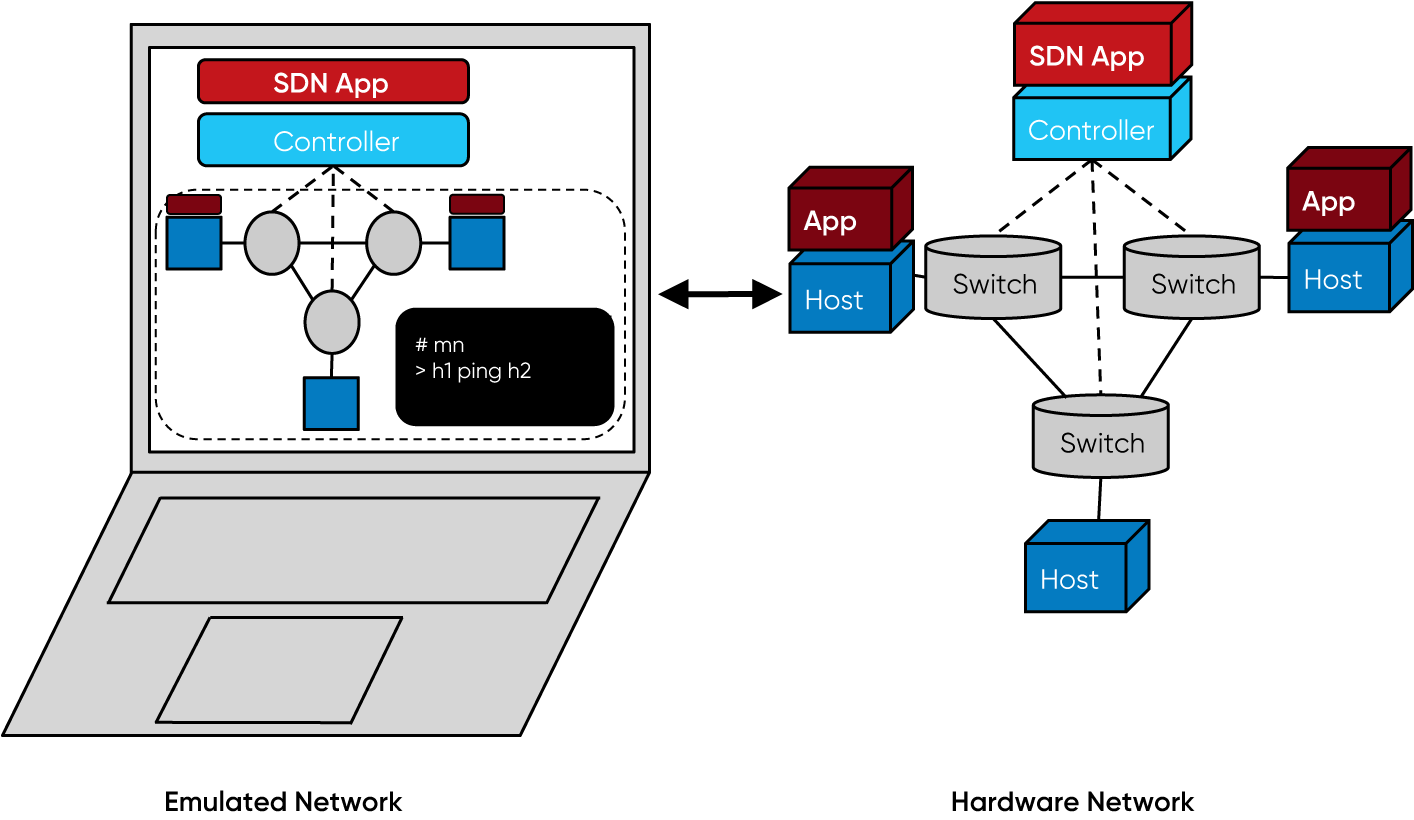
\includegraphics[scale=0.145]{images/mininet-what-is-mininet.png}
      %  \caption{A figure that is next to a certain explanation.}
      \end{figure}
    \end{column}
  \end{columns}
\end{frame}

%------------------------------------------------------------------------------%
\begin{frame}
  \frametitle{A Mininet network consists of:}

  \begin{block}{\textbf{Isolated Hosts}} 
    A group of user-level processes moved into a network namespace
    that provide exclusive ownership of interfaces, ports and routing
    tables.
  \end{block}

\end{frame}
%------------------------------------------------------------------------------%
\begin{frame}
  \frametitle{A Mininet network consists of:}

  \begin{block}{\textbf{Isolated Hosts}} 
    A group of user-level processes moved into a network namespace
    that provide exclusive ownership of interfaces, ports and routing
    tables.
  \end{block}
  \begin{block}{\textbf{Emulated Switches}} 
    The default Linux Bridge or the Open vSwitch running in kernel
    mode is used to switch packets across interfaces. Switches and
    routers can run in the kernel or in the user space.
  \end{block}

\end{frame}
%------------------------------------------------------------------------------%
%------------------------------------------------------------------------------%
\begin{frame}
  \frametitle{A Mininet network consists of:}

  \begin{block}{\textbf{Isolated Hosts}} 
    A group of user-level processes moved into a network namespace
    that provide exclusive ownership of interfaces, ports and routing
    tables.
  \end{block}
  \begin{block}{\textbf{Emulated Links}} 
    Each emulated host has its own virtual Ethernet interface(s).
    Linux Traffic Control \textit{tc} enforces the data rate of each link
    to shape traffic to a configured rate.
  \end{block}
  \begin{block}{\textbf{Emulated Switches}} 
    The default Linux Bridge or the Open vSwitch running in kernel
    mode is used to switch packets across interfaces. Switches and
    routers can run in the kernel or in the user space.
  \end{block}

\end{frame}
%------------------------------------------------------------------------------%
\begin{frame}
  \frametitle{Why use Mininet?}
  \begin{itemize}
    \item[\ding{219}] \textbf{It's fast}
      
      Starting up a simple network takes just a few seconds.
  \end{itemize}
\end{frame}
\begin{frame}
  \frametitle{Why use Mininet?}
  \begin{itemize}
    \item[\ding{219}] It's fast
    \item[\ding{219}] \textbf{You can create custom topologies}

      A single switch, larger Internet-like topologies, a data center,
      or anything else.
  \end{itemize}
\end{frame}
\begin{frame}
  \frametitle{Why use Mininet?}
  \begin{itemize}
    \item[\ding{219}] It's fast
    \item[\ding{219}] You can create custom topologies
    \item[\ding{219}] \textbf{You can run real programs}

      Anything that runs on Linux is available for you to run, from
      web servers to TCP window monitoring tools to Wireshark.
  \end{itemize}
\end{frame}
\begin{frame}
  \frametitle{Why use Mininet?}
  \begin{itemize}
    \item[\ding{219}] It's fast
    \item[\ding{219}] You can create custom topologies
    \item[\ding{219}] You can run real programs
    \item[\ding{219}] \textbf{You can run Mininet everywhere}

      On your laptop, on a server, in a VM, on a native Linux box
      (Mininet is included with Ubuntu 12.10+!), or in the cloud (e.g.
      Amazon EC2.)
  \end{itemize}
\end{frame}
\begin{frame}
  \frametitle{Why use Mininet?}
  \begin{itemize}
    \item[\ding{219}] It's fast
    \item[\ding{219}] You can create custom topologies
    \item[\ding{219}] You can run real programs
    \item[\ding{219}] You can run Mininet everywhere
    \item[\ding{219}] \textbf{You can share and replicate results}

      Anyone with a computer can run your code.
  \end{itemize}
\end{frame}
\begin{frame}
  \frametitle{Why use Mininet?}
  \begin{itemize}
    \item[\ding{219}] It's fast
    \item[\ding{219}] You can create custom topologies
    \item[\ding{219}] You can run real programs
    \item[\ding{219}] You can run Mininet everywhere
    \item[\ding{219}] You can share and replicate results
    \item[\ding{219}] \textbf{You can use it easily}

      You can create and run Mininet experiments by writing simple (or
      complex if necessary) Python scripts.
  \end{itemize}
\end{frame}
\begin{frame}
  \frametitle{Why use Mininet?}
  \begin{itemize}
    \item[\ding{219}] It's fast
    \item[\ding{219}] You can create custom topologies
    \item[\ding{219}] You can run real programs
    \item[\ding{219}] You can run Mininet everywhere
    \item[\ding{219}] You can share and replicate results
    \item[\ding{219}] You can use it easily
    \item[\ding{219}] \textbf{Mininet is an open source project}

      \url{https://github.com/mininet}
  \end{itemize}
\end{frame}

%------------------------------------------------------------------------------%
\begin{frame}
  \frametitle{Installation and Setup}

  \begin{block}{\textbf{1. Mininet VM Installation}}
    Download a Mininet VM Image from
    \url{https://github.com/mininet/mininet/releases/}
  \end{block}

\end{frame}
%------------------------------------------------------------------------------%
\begin{frame}[fragile]
  \frametitle{Installation and Setup}

  \begin{block}{1. Mininet VM Installation}
  \end{block}
  \begin{block}{\textbf{2. Native Installation from Source}}
    \rule{\textwidth}{0.5pt}
    \small
    \begin{minted}{bash}
    # Get the source code
    git clone https://github.com/mininet/mininet
    # Run the following command to install Mininet
    mininet/util/install.sh [options]
  \end{minted}
  \rule{\textwidth}{0.5pt}
\end{block}
\end{frame}
%------------------------------------------------------------------------------%
%------------------------------------------------------------------------------%
\begin{frame}[fragile]
  \frametitle{Installation and Setup}

  \begin{block}{1. Mininet VM Installation}
  \end{block}
  \begin{block}{2. Native Installation from Source}
  \end{block}
  \begin{block}{\textbf{3. Installation from Packages}}
    \rule{\textwidth}{0.5pt}
    \small
\begin{minted}{bash}
     # Install the base Mininet package
     sudo apt install mininet
     # Test Open vSwitch
     sudo mn --switch ovsbr --test pingall
     # Make sure Open vSwitch is installed
     sudo apt-get install openvswitch-switch
     sudo service openvswitch-switch start
\end{minted}
    \rule{\textwidth}{0.5pt}
  \end{block}
\end{frame}
%------------------------------------------------------------------------------%
\begin{frame}
  \frametitle{Hands-on Demo Session}
  \begin{block}{Instructions at:}

    \url{https://github.com/kristjoc/org-mininet/}
  \end{block}
\end{frame}
%------------------------------------------------------------------------------%
\begin{frame}[plain]
  \begin{itemize}
  \item[] {\color{gray}Mininet Walkthrough}
    \vspace{1cm}
  \item[]
    \begin{large}
      Mininet Python API
    \end{large}
    \vspace{1cm}
  \item[] {\color{gray}Mininet and SDN}
  \end{itemize}
  \addtocounter{framenumber}{-1}
\end{frame}
%------------------------------------------------------------------------------%
\begin{frame}[fragile]
  \frametitle{Mininet Python API}

  \begin{block}{Defining Custom Topologies through Python API}
    \rule{0.5\textwidth}{0.5pt}
    \scriptsize
\begin{minted}{python}
    from mininet.topo import Topo

    class MyTopo( Topo ):
        "Simple topology example."

        def build( self ):
            # Add hosts and switches
            leftHost = self.addHost( 'h1' )
            rightHost = self.addHost( 'h2' )
            leftSwitch = self.addSwitch( 's3' )
            rightSwitch = self.addSwitch( 's4' )

            # Add links
            self.addLink( leftHost, leftSwitch )
            self.addLink( leftSwitch, rightSwitch )
            self.addLink( rightSwitch, rightHost )

    topos = { 'mytopo': ( lambda: MyTopo() ) }
\end{minted}
    \rule{0.5\textwidth}{0.5pt}
  \end{block}
\end{frame}
%------------------------------------------------------------------------------%
\begin{frame}
  \frametitle{Mininet Python API}

  \begin{block}{\textbf{1. Low-level API}}
    The low-level API consists of the base node and link classes (such
    as \textit{Host}, \textit{Switch}, and \textit{Link} and their
    subclasses) which can actually be instantiated individually and
    used to create a network.
  \end{block}
\end{frame}

\begin{frame}[fragile]
  \frametitle{Mininet Python API}

  \begin{block}{\textbf{1. Low-level API: Nodes and Links}}
    \rule{0.5\textwidth}{0.5pt}
    \footnotesize
\begin{minted}{python}
  h1 = Host( 'h1' )
  h2 = Host( 'h2' )
  s1 = OVSSwitch( 's1', inNamespace=False )
  c0 = Controller( 'c0', inNamespace=False )
  Link( h1, s1 )
  Link( h2, s1 )
  h1.setIP( '10.1/8' )
  h2.setIP( '10.2/8' )
  c0.start()
  s1.start( [ c0 ] )
  print( h1.cmd( 'ping -c1', h2.IP() ) )
  s1.stop()
  c0.stop()
\end{minted}
    \rule{0.5\textwidth}{0.5pt}
  \end{block}
\end{frame}

%------------------------------------------------------------------------------%
\begin{frame}
  \frametitle{Mininet Python API}

  \begin{block}{1. Low-level API}
  \end{block}
  \begin{block}{\textbf{2. Mid-level API}}
    The mid-level API adds the \textit{Mininet} object which serves as
    a container for nodes and links. It provides a number of methods
    (such as \textit{addHost()}, \textit{addSwitch()}, and
    \textit{addLink()}) for adding nodes and links to a network, as
    well as network configuration, startup and shutdown (notably
    \textit{start()} and \textit{stop()}.)
\end{block}
\end{frame}
\begin{frame}[fragile]
  \frametitle{Mininet Python API}

  \begin{block}{1. Low-level API}
  \end{block}
  \begin{block}{\textbf{2. Mid-level API: Network object}}
    \rule{0.5\textwidth}{0.5pt}
    \footnotesize
\begin{minted}{python}
  net = Mininet()
  h1 = net.addHost( 'h1' )
  h2 = net.addHost( 'h2' )
  s1 = net.addSwitch( 's1' )
  c0 = net.addController( 'c0' )
  net.addLink( h1, s1 )
  net.addLink( h2, s1 )
  net.start()
  print( h1.cmd( 'ping -c1', h2.IP() ) )
  CLI( net )
  net.stop()
\end{minted}
    \rule{0.5\textwidth}{0.5pt}
\end{block}
\end{frame}

\begin{frame}[fragile]
  \frametitle{Mininet Python API}

  \begin{block}{1. Low-level API}
  \end{block}
  \begin{block}{2. Mid-level API}
  \end{block}
  \begin{block}{\textbf{3. High-level API}}
    The high-level API adds a topology template abstraction, the
    \textit{Topo} class, which provides the ability to create
    reusable, parametrized topology templates. These templates can be
    passed to the \textit{mn} command (via the \textit{--custom}
    option) and used from the command line.
\begin{minted}{bash}
sudo mn --custom custom_example.py --topo mytopo
\end{minted}    
  \end{block}
\end{frame}
%------------------------------------------------------------------------------%
\begin{frame}[fragile]
  \frametitle{Mininet Python API}

  \begin{block}{1. Low-level API}
  \end{block}
  \begin{block}{2. Mid-level API}
  \end{block}
  \begin{block}{\textbf{3. High-level API: Topology templates}}
    \rule{0.5\textwidth}{0.5pt}
    \scriptsize
\begin{minted}{python}
  class SingleSwitchTopo( Topo ):
      def build( self, count=1 ):
          hosts = [ self.addHost( 'h%d' % i )
                    for i in range( 1, count + 1 ) ]
          s1 = self.addSwitch( 's1' )
          for h in hosts:
              self.addLink( h, s1 )

  net = Mininet( topo=SingleSwitchTopo( 3 ) )
  net.start()
  CLI( net )
  net.stop()
\end{minted}
    \rule{0.5\textwidth}{0.5pt}
  \end{block}
\end{frame}
\begin{frame}[fragile]
  \frametitle{Mininet Python API}

  \begin{block}{Mininet API Documentation}
    \rule{\textwidth}{0.5pt}
    \footnotesize
\begin{minted}{python}
  python
  >>> from mininet.node import Host
  >>> help(Host.IP)
  Help on method IP in module mininet.node:

  IP(self, intf=None) unbound mininet.node.Host method
          Return IP address of a node or specific interface.
\end{minted}
    \rule{\textwidth}{0.5pt}
\end{block}
\end{frame}

%------------------------------------------------------------------------------%
\begin{frame}
  \frametitle{Hands-on Demo Session}
  \begin{block}{Instructions at:}
    \centering
    \url{https://github.com/kristjoc/org-mininet/}
  \end{block}
\end{frame}

%------------------------------------------------------------------------------%
\begin{frame}[plain]
  \begin{itemize}
  \item[] {\color{gray}Mininet Walkthrough}
    \vspace{1cm}
  \item[] {\color{gray}Mininet Python API}
    \vspace{1cm}
  \item[]
    \begin{large}
      Mininet and SDN
    \end{large}
  \end{itemize}
  \addtocounter{framenumber}{-1}
\end{frame}
%------------------------------------------------------------------------------%
%------------------------------------------------------------------------------%

\begin{frame}
  \frametitle{First, networks are enormous in size}
  \begin{figure}
    \begin{center}
      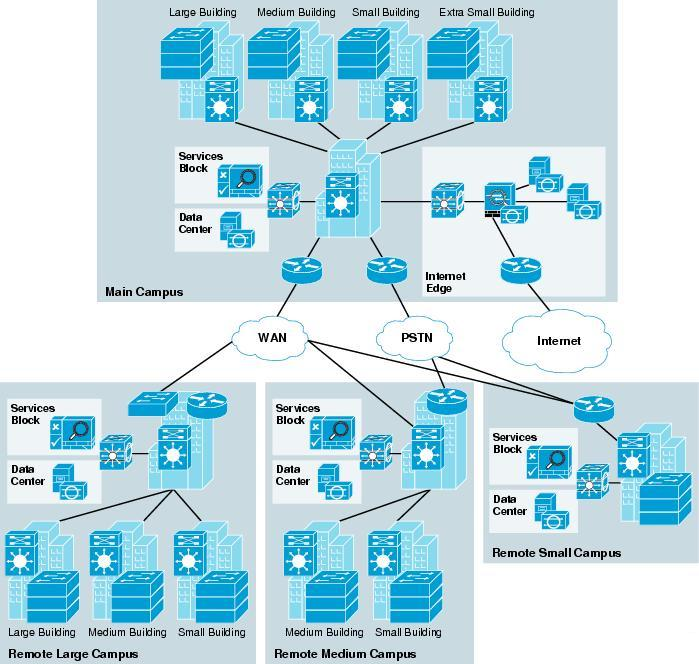
\includegraphics[scale=0.25]{images/sdn-1}
    \end{center}
    
    \caption{\small{[Photo: Cisco]}}
  \end{figure}
\end{frame}
%------------------------------------------------------------------------------%
\begin{frame}
  \frametitle{Second, networks are highly heterogeneous}
  \begin{figure}
    \begin{center}
      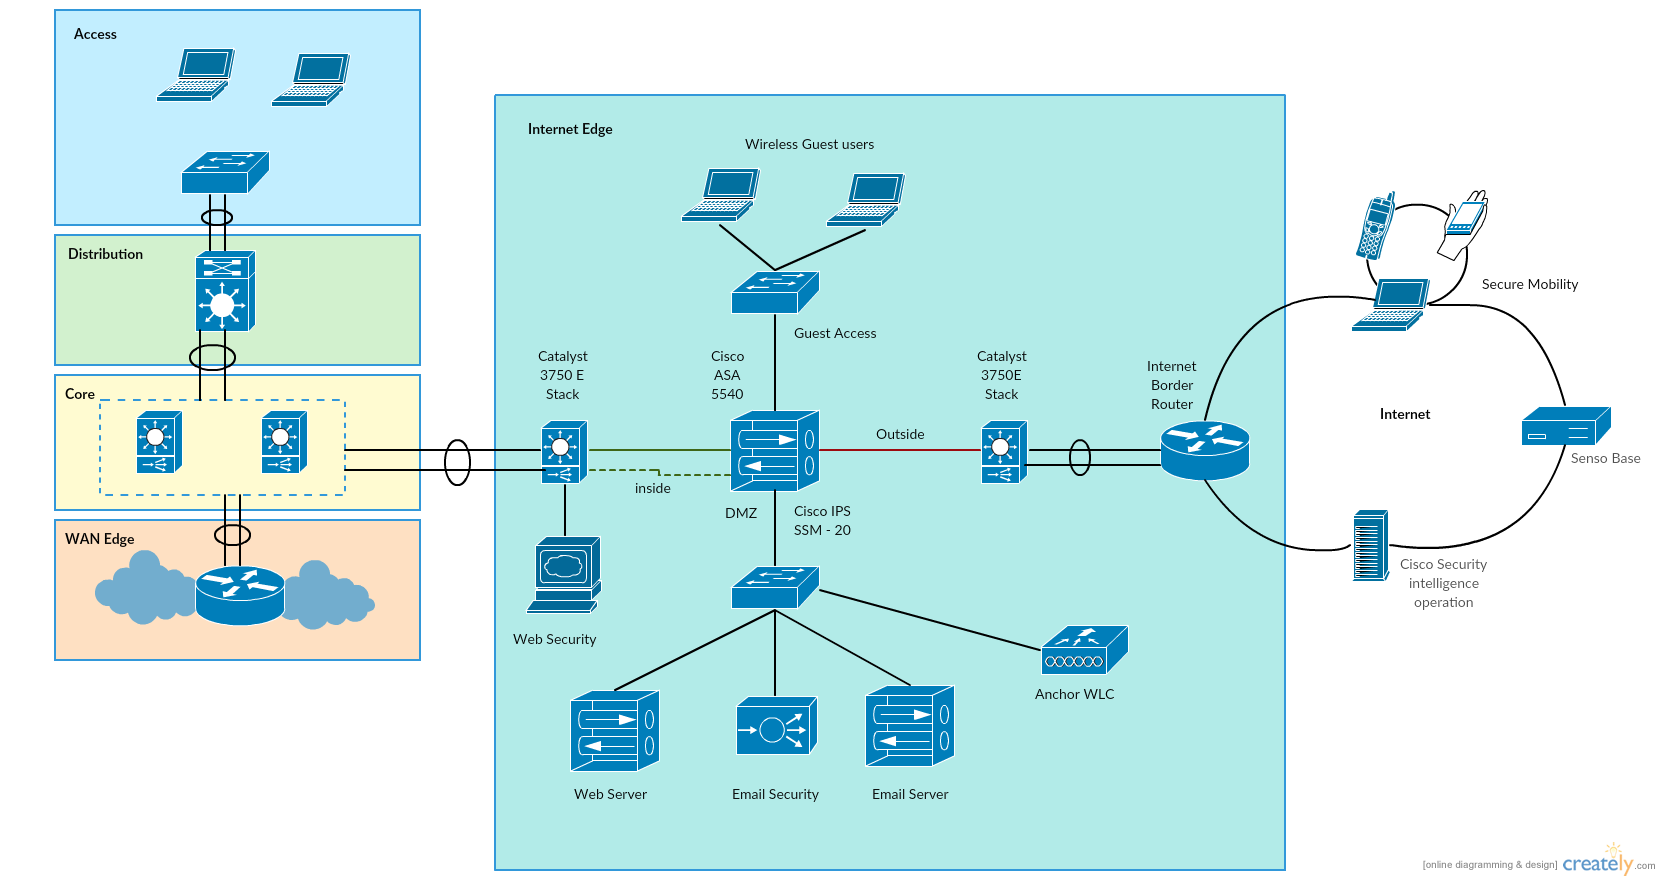
\includegraphics[scale=0.25]{images/sdn-2}
    \end{center}
    
    \caption{\small{[Photo: Google Images]}}
  \end{figure}
\end{frame}
\begin{frame}
  \frametitle{Second, networks are highly heterogeneous}
  \begin{figure}
    \begin{center}
      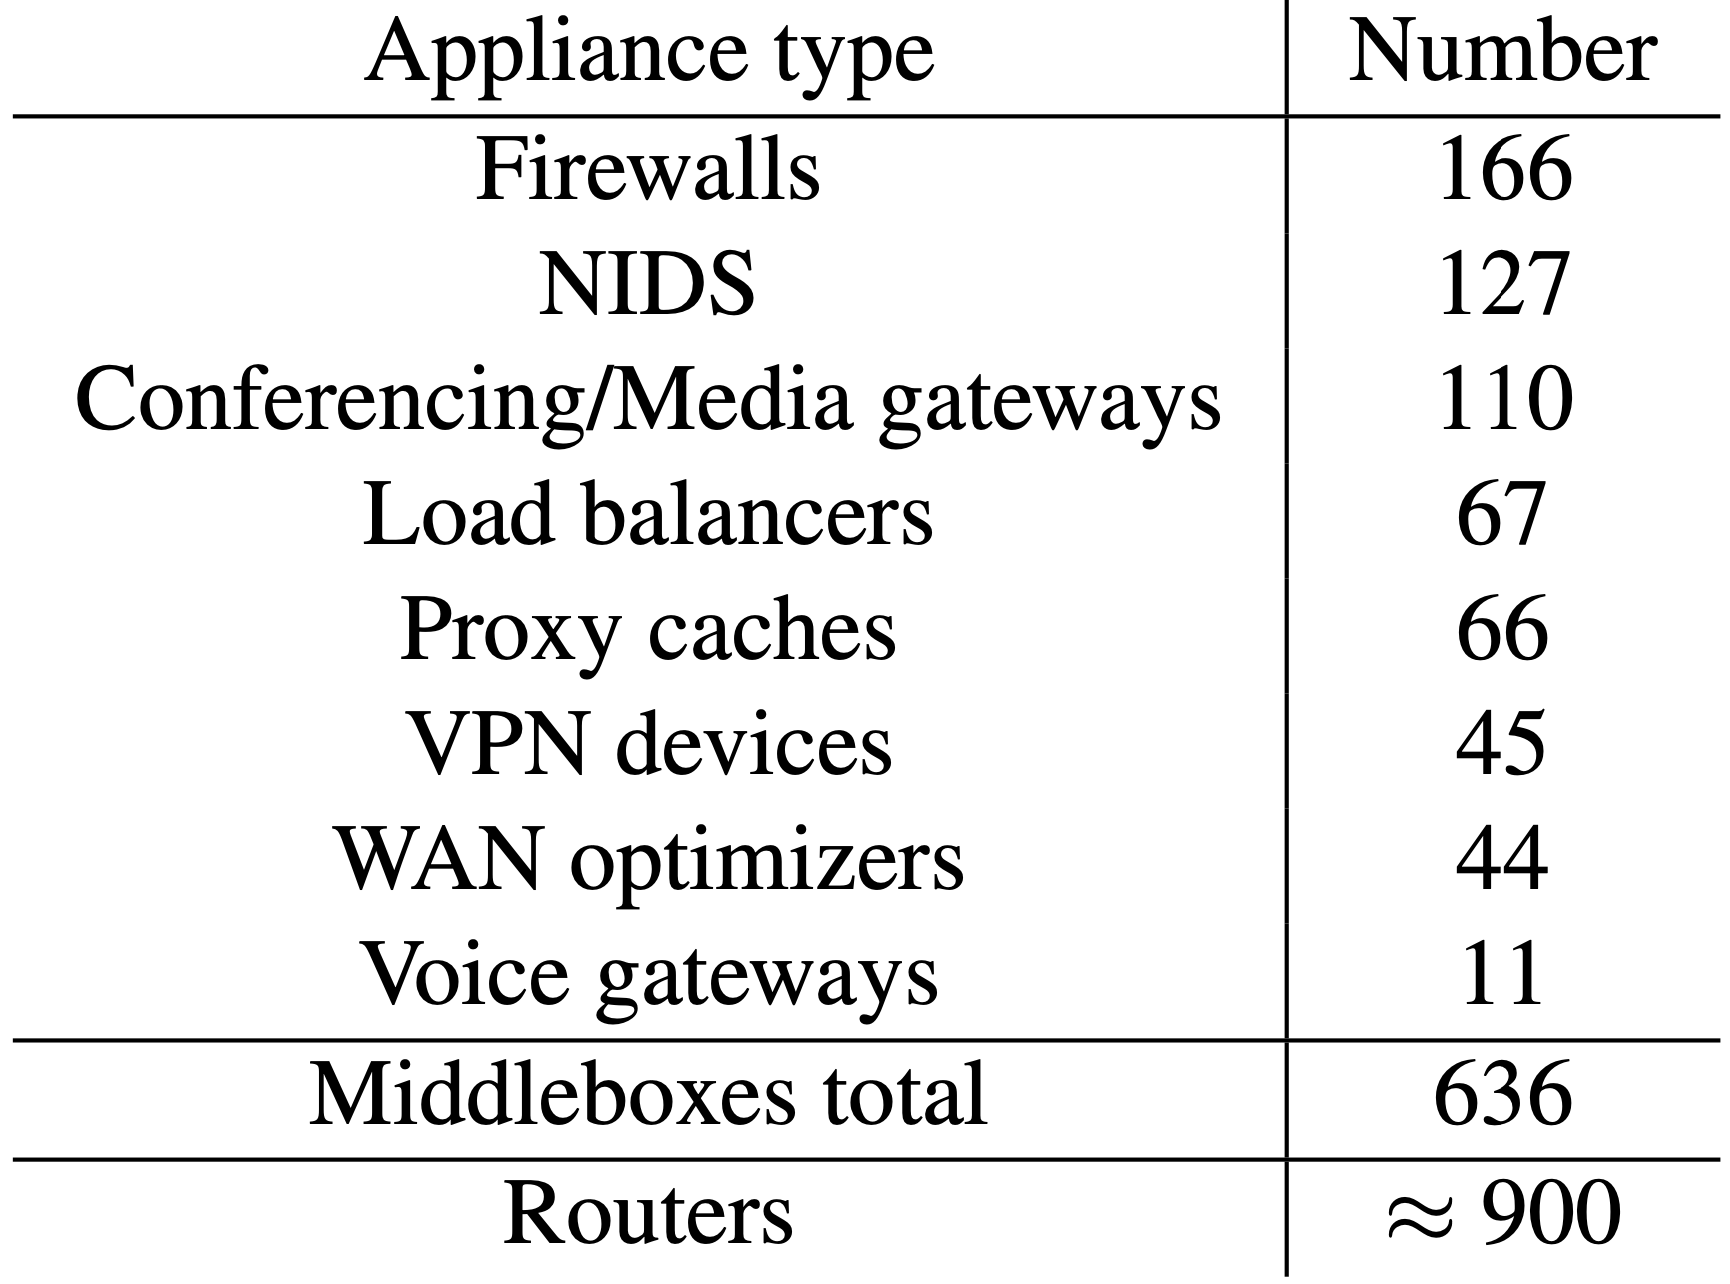
\includegraphics[scale=0.25]{images/sdn-3}
    \end{center}
    
    \caption{\small{[ Source: Sekar et al, Design and Implementation of a Consolidated Middlebox Architecture, NSDI 12 ]}}
  \end{figure}
\end{frame}
\begin{frame}
  \frametitle{Third, networks are very complex to manage}
  \begin{figure}
    \begin{center}
      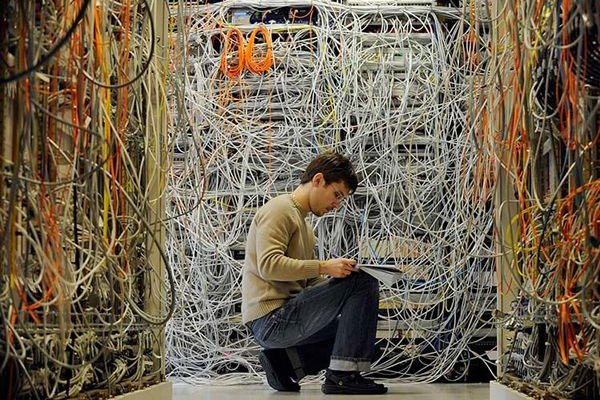
\includegraphics[scale=0.25]{images/sdn-4}
    \end{center}
    
    \caption{\small{[ Photo: Google Images ]}}
  \end{figure}
\end{frame}
\begin{frame}
  \frametitle{Third, networks are very complex to manage}
  \begin{figure}
    \begin{center}
      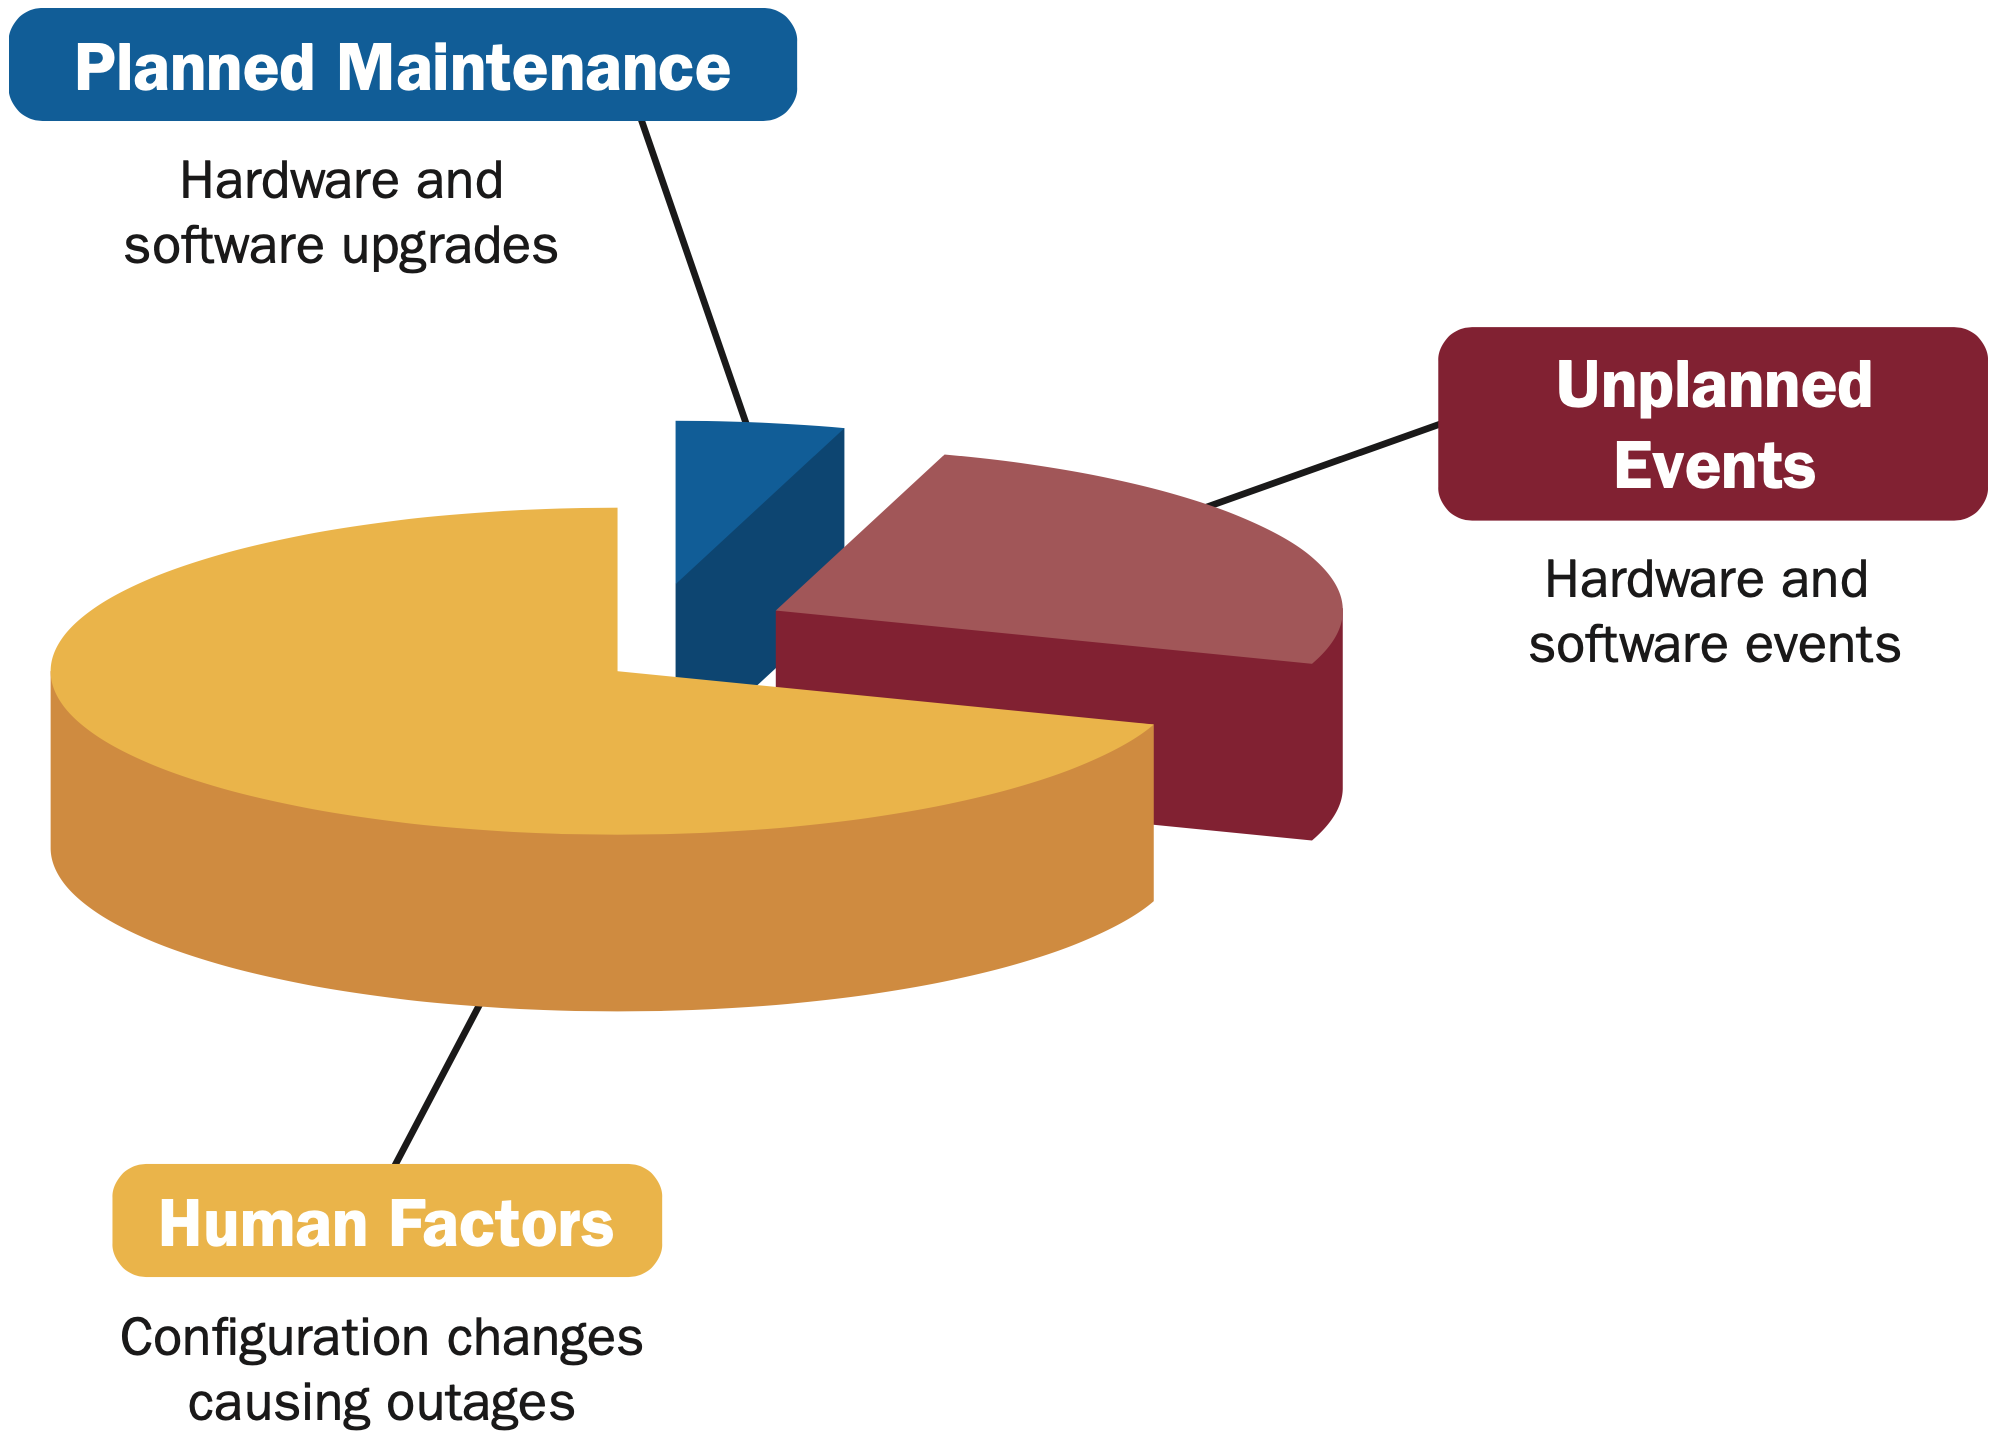
\includegraphics[scale=0.25]{images/sdn-5}
    \end{center}
    
    \caption{\small{[ Photo: Juniper ]}}
  \end{figure}
\end{frame}
\begin{frame}
  \frametitle{Third, networks are very complex to manage}
  \begin{figure}
    \begin{center}
      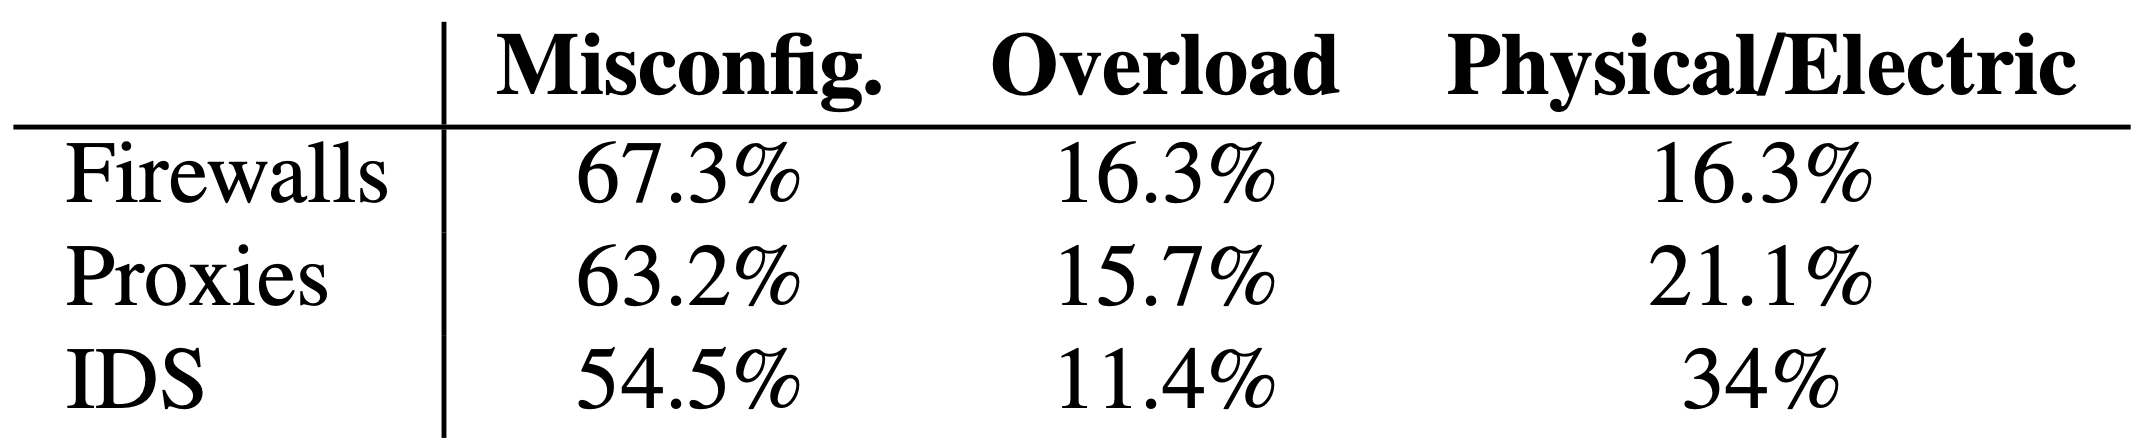
\includegraphics[scale=0.25]{images/sdn-6}
    \end{center}
    
    \caption{\small{[ Source: Sherry et al, Making Middleboxes Someone Else's Problem:
                                  Network Processing as a Cloud Service, SIGGCOM 12 ]}}
  \end{figure}
\end{frame}


\begin{frame}[plain]
  \begin{center}
  \large What is Software-Defined Networking (SDN)?
  \end{center}
  \addtocounter{framenumber}{-1}
\end{frame}

\begin{frame}
  \frametitle{What is SDN?}

  \begin{block}{}
    \centering

    Physical separation of the network control plane from the
    forwarding plane
    
  \end{block}
  \begin{block}{}
    \centering
    The control plane controls several devices and is directly
    programmable
  \end{block}

\end{frame}

\begin{frame}
  \frametitle{Network planes (Mgmt., Control, and Data planes)}
  \begin{figure}
    \begin{center}
      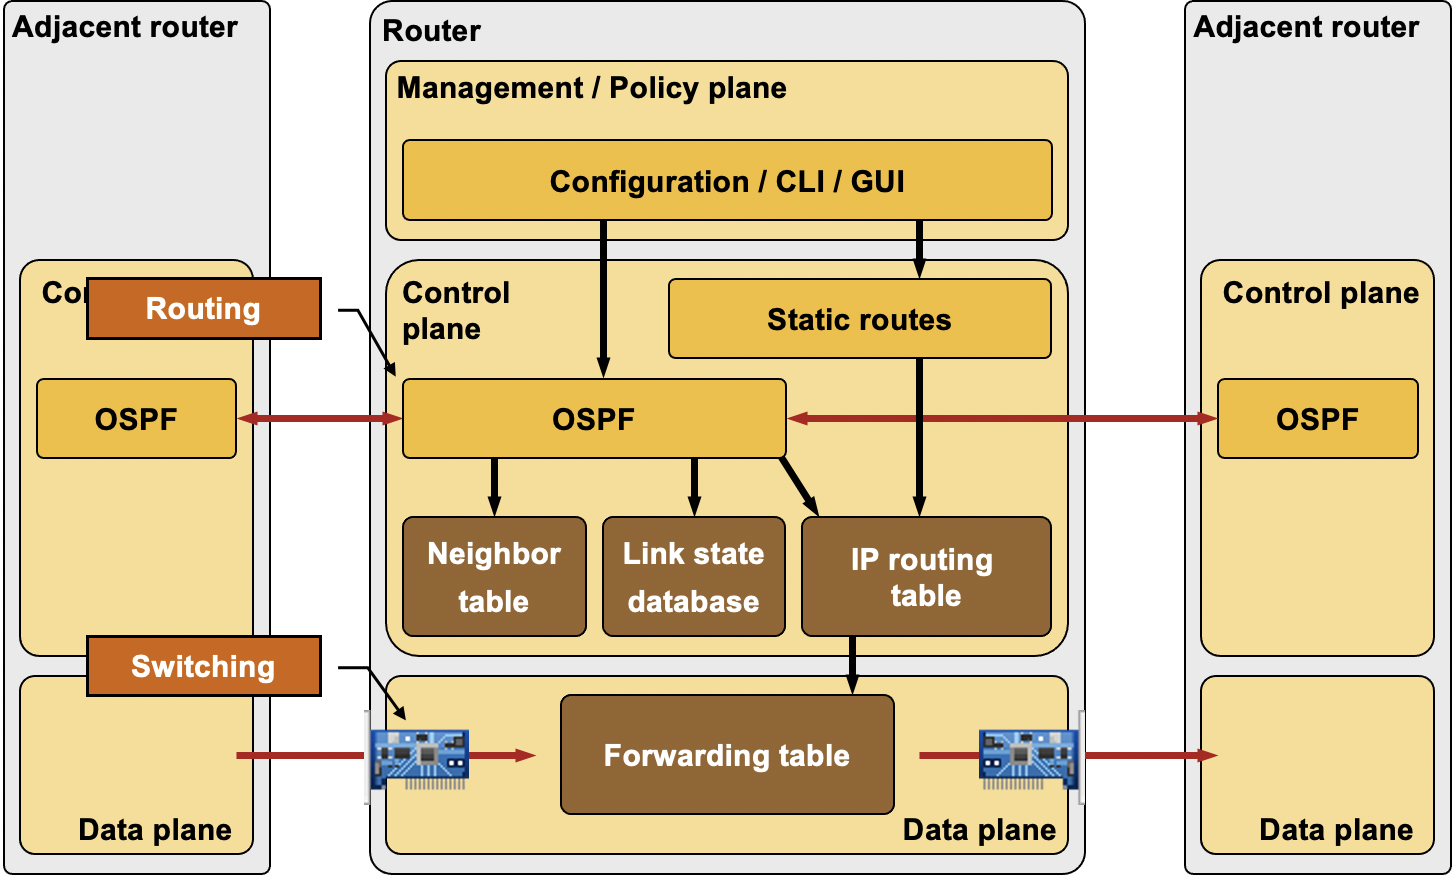
\includegraphics[scale=0.2]{images/sdn-7}
    \end{center}
    
    \caption{\small{[ Photo: ipSpace.net ]}}
  \end{figure}
\end{frame}
\begin{frame}
  \frametitle{In traditional networking, Control and Data planes
    reside within the physical device}
  \begin{figure}
    \begin{center}
      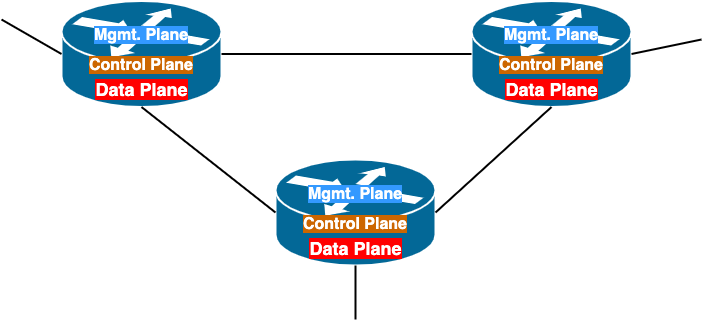
\includegraphics[scale=0.45]{images/sdn-8}
    \end{center}
  \end{figure}
\end{frame}
\begin{frame}
  \frametitle{SDN: Separation of Control and Data planes}
  \begin{figure}
    \begin{center}
      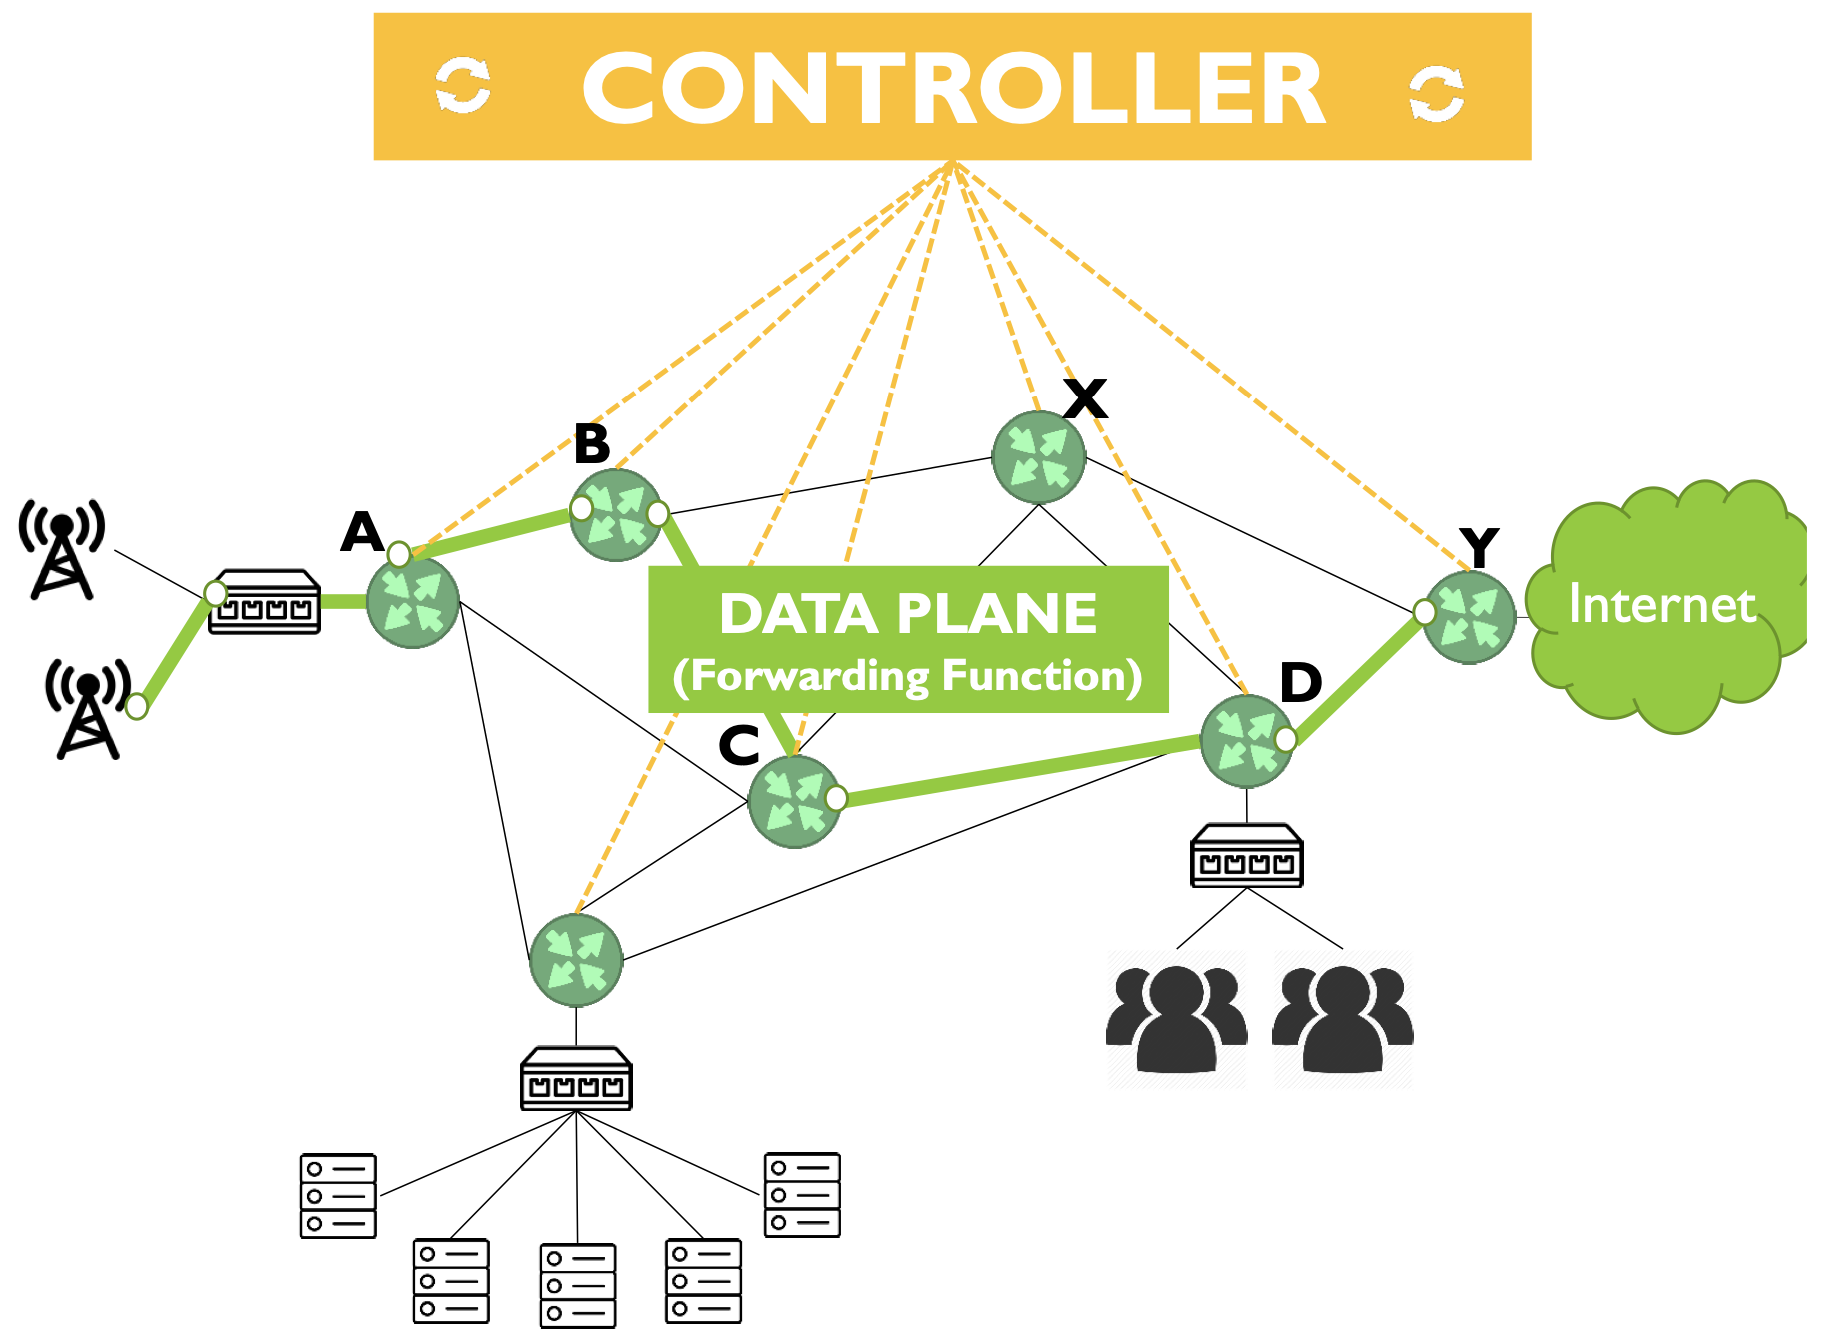
\includegraphics[scale=0.275]{images/sdn-9}
    \end{center}
    \vspace{-0.05cm}
    \caption{\small{[ Photo: TelecomTutorial.org ]}}
  \end{figure}
\end{frame}

%------------------------------------------------------------------------------%
\begin{frame}
  \frametitle{What are the benefits of SDN?}
\end{frame}

%------------------------------------------------------------------------------%
\begin{frame}
  \frametitle{What are the benefits of SDN?}
      \begin{itemize}[<+->]
      \item[\ding{219}] Directly programmable
      \item[\ding{219}] Agile
      \item [\ding{219}] Centrally managed
      \item [\ding{219}] Open Standard based
      \item [\ding{219}] Vendor-neutral
    \end{itemize}
\end{frame}
\begin{frame}
  \frametitle{What are the challenges of SDN?}
\end{frame}

%------------------------------------------------------------------------------%
\begin{frame}
  \frametitle{What are the challenges of SDN?}
      \begin{itemize}[<+->]
      \item[\ding{219}] Standardization and Adoption
      \item[\ding{219}] Reliability
      \item [\ding{219}] Performance
      \item [\ding{219}] Scalability
      \item [\ding{219}] Security
    \end{itemize}
\end{frame}


\begin{frame}
  \frametitle{SDN Architecture}
  \begin{figure}
    \begin{center}
      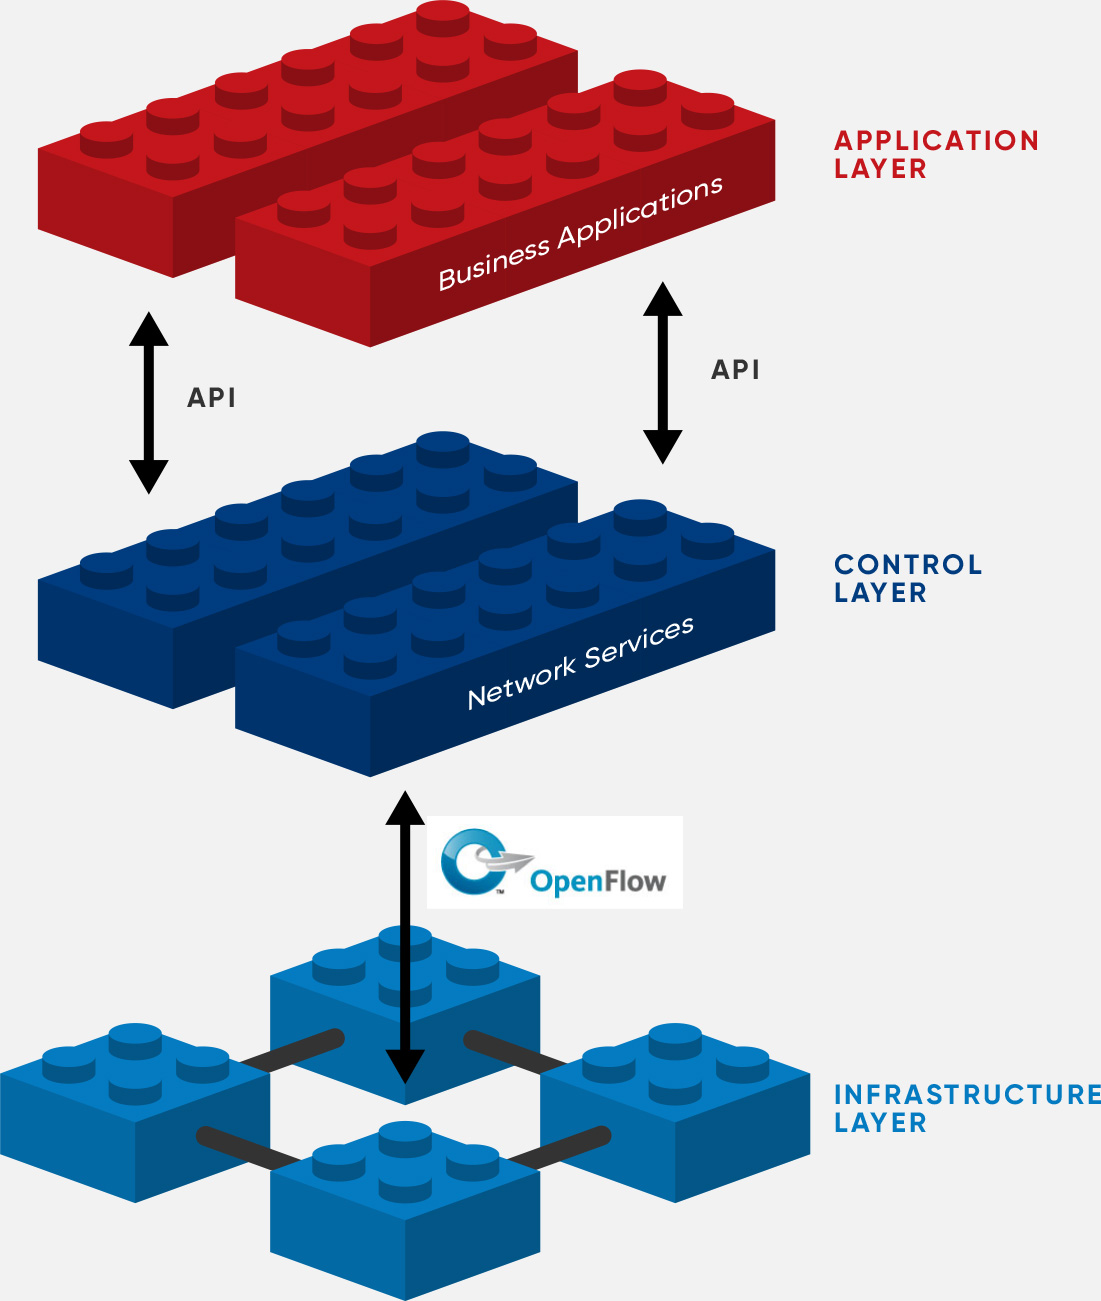
\includegraphics[scale=0.125]{images/sdn-10}
    \end{center}
    \vspace{0.5cm}
    \caption{\small{[ Photo: Open Networking Foundation ]}}
  \end{figure}
\end{frame}
%------------------------------------------------------------------------------%
\begin{frame}
  \frametitle{SDN Infrastructure Layer}
  \begin{figure}
    \begin{center}
      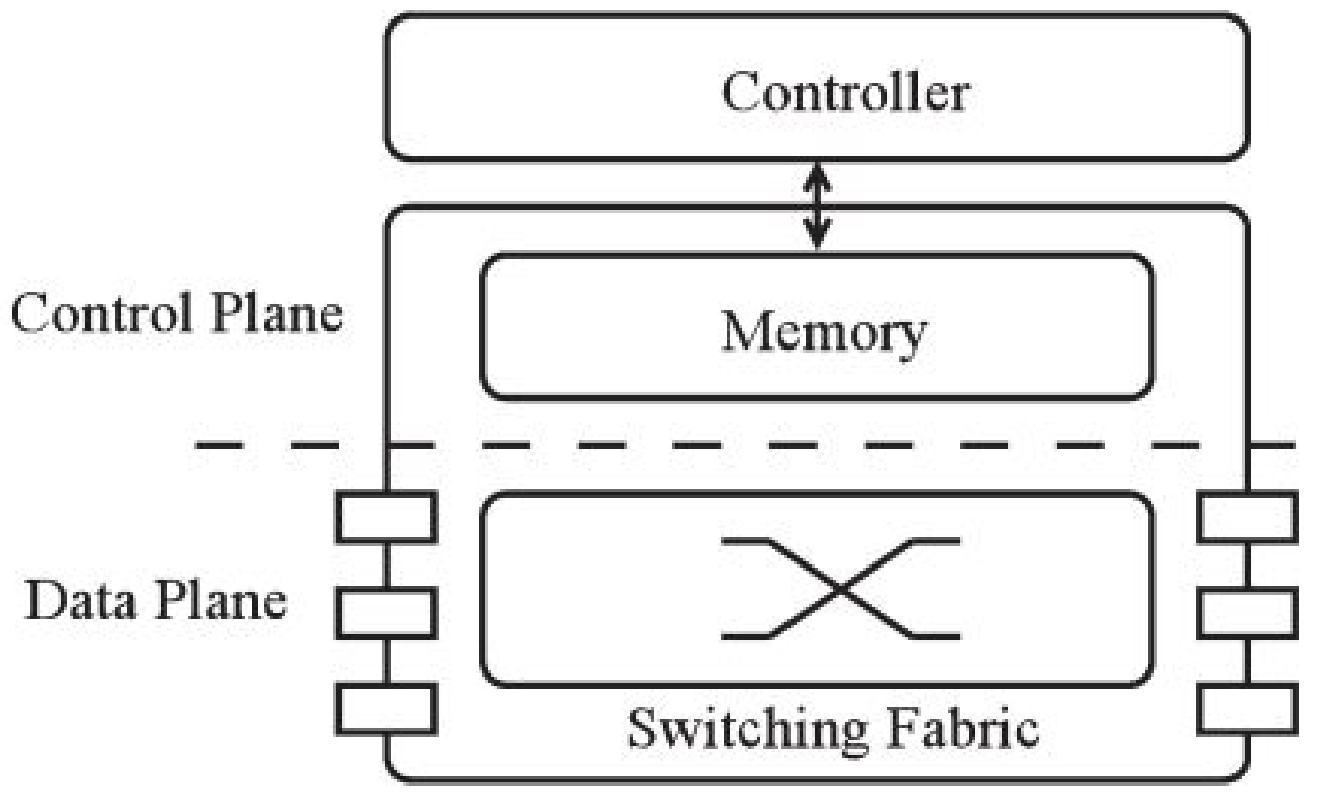
\includegraphics[scale=0.3]{images/sdn-11}
    \end{center}
    \vspace{0.5cm}
    \caption{\small{[ Source: Xia et al, A Survey on Software-Defined Networking, IEEE COMST 14 ]}}
  \end{figure}
\end{frame}
\begin{frame}
  \frametitle{SDN Control Layer}
  \begin{figure}
    \begin{center}
      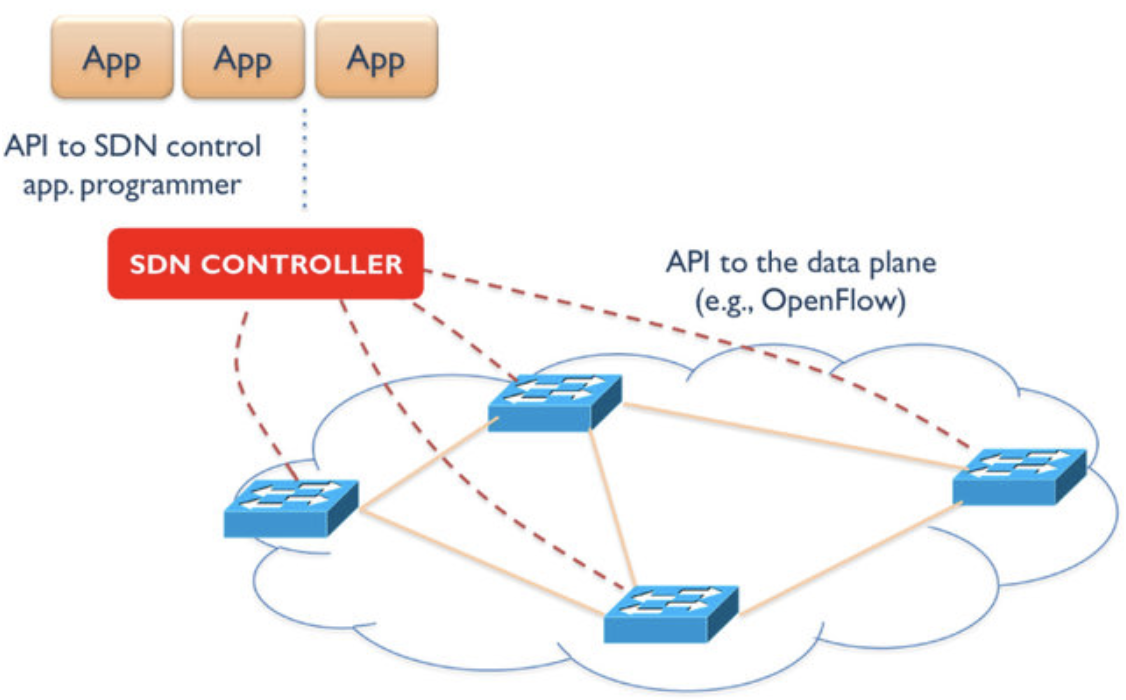
\includegraphics[scale=0.5]{images/sdn-12}
    \end{center}
    \caption{\small{[ Source: ResearchGate ]}}
  \end{figure}
\end{frame}
\begin{frame}
  \frametitle{SDN Control Layer}
  \begin{figure}
    \begin{center}
      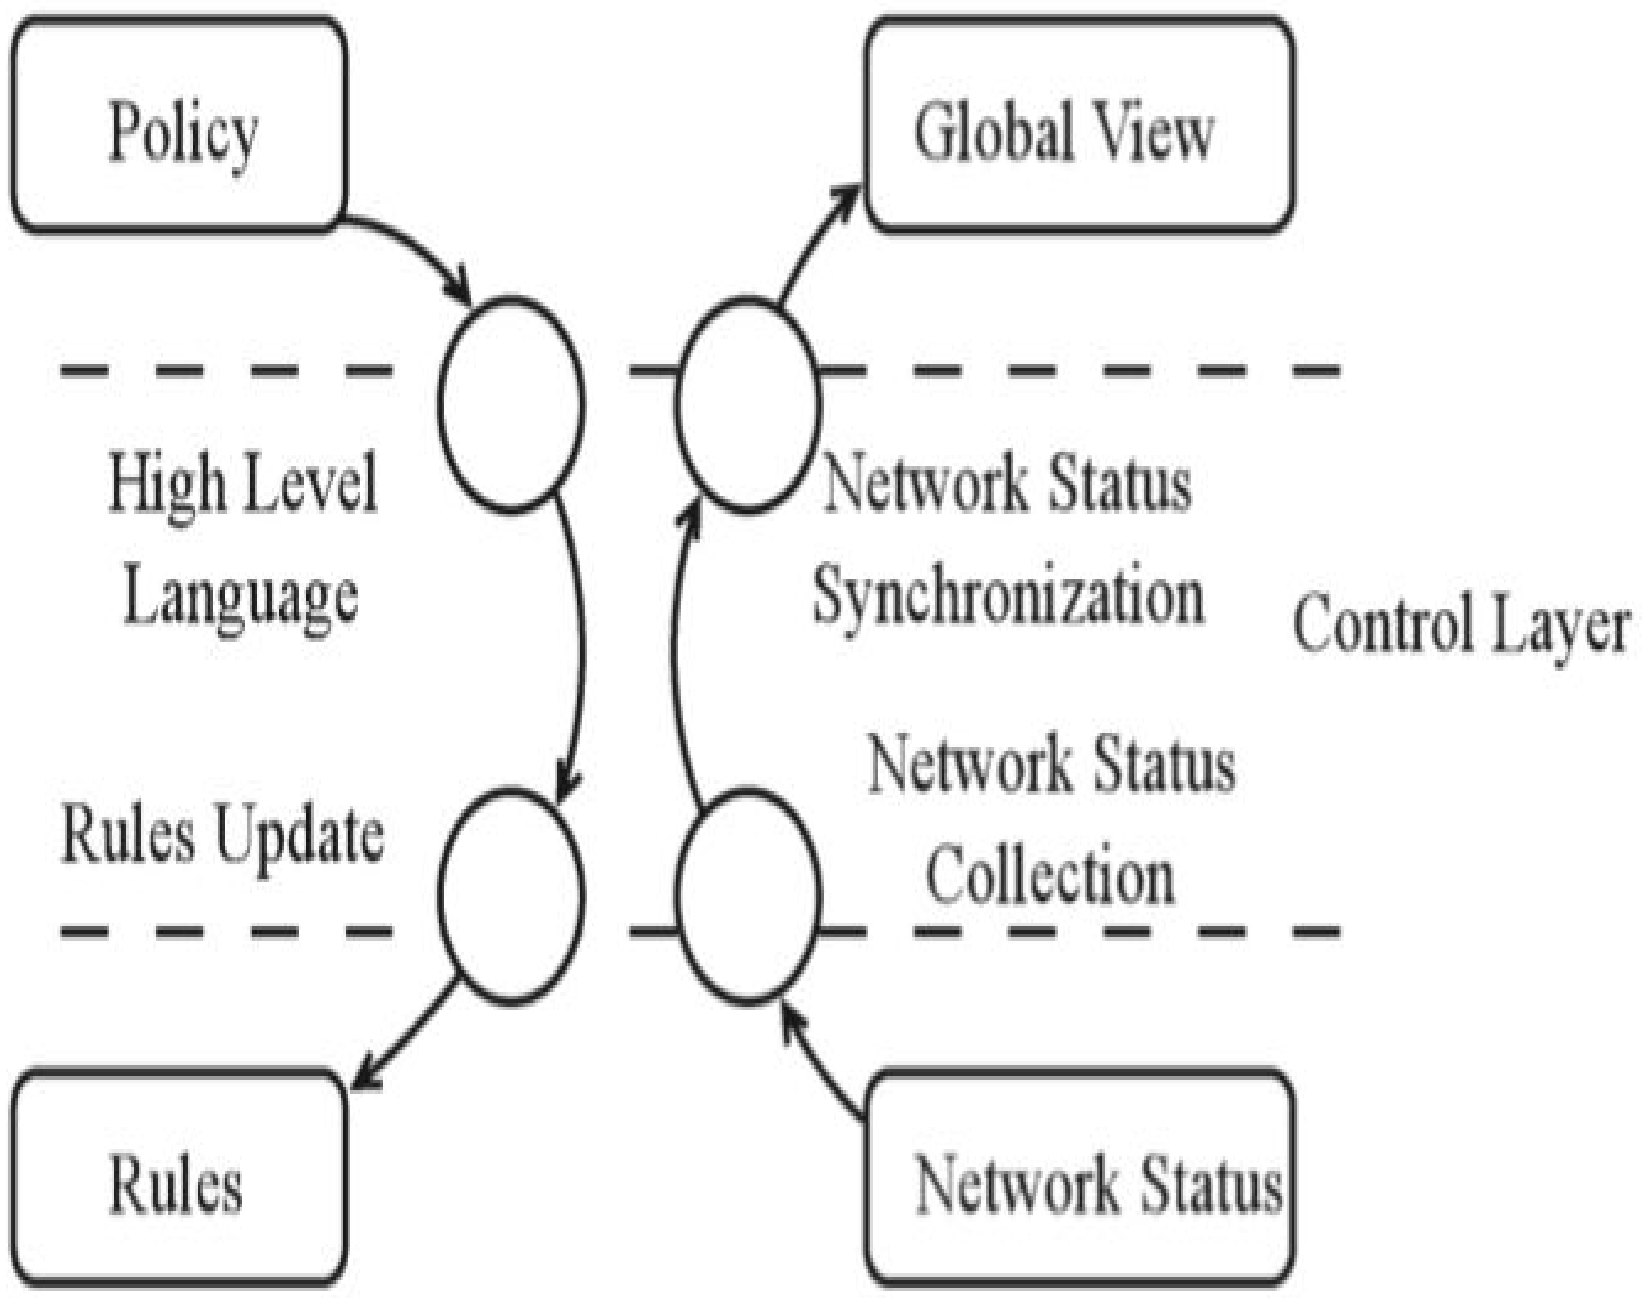
\includegraphics[scale=0.25]{images/sdn-13}
    \end{center}
    \vspace{0.5cm}
    \caption{\small{[ Source: Xia et al, A Survey on Software-Defined Networking, IEEE COMST 14 ]}}
  \end{figure}
\end{frame}
\begin{frame}
  \frametitle{OpenFlow Protocol}
  \begin{figure}
    \begin{center}
      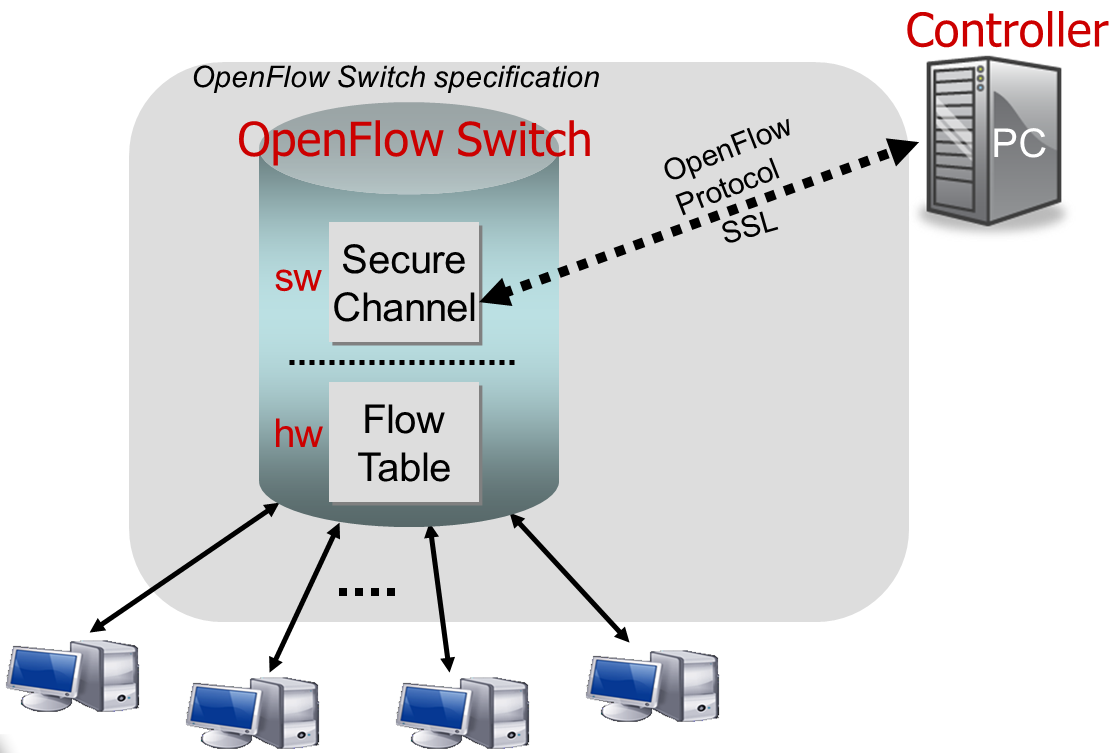
\includegraphics[scale=0.25]{images/sdn-14}
    \end{center}
    \caption{\small{[ Source: slideshare.net ]}}
  \end{figure}
\end{frame}
\begin{frame}
  \frametitle{OpenFlow Protocol}
  \begin{figure}
    \begin{center}
      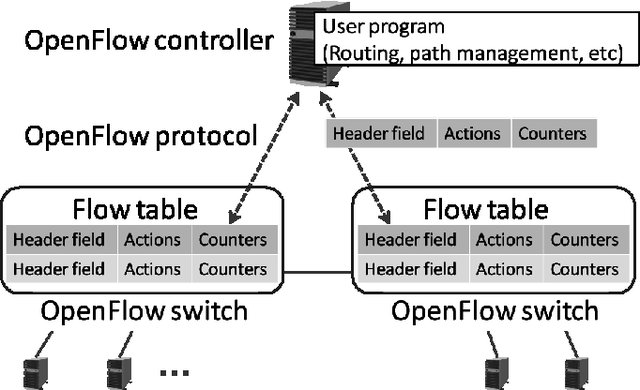
\includegraphics[scale=0.95]{images/sdn-15}
    \end{center}
    \vspace{1cm}
    \caption{\small{[Source: Suzuki et al, A Survey on OpenFlow Technologies, IEICE ToC, 14]}}
  \end{figure}
\end{frame}

\begin{frame}
  \frametitle{SDN Application Layer}
  \begin{columns}
    % Column 1
    \begin{column}{0.55\textwidth}
      \begin{figure}
        \centering
        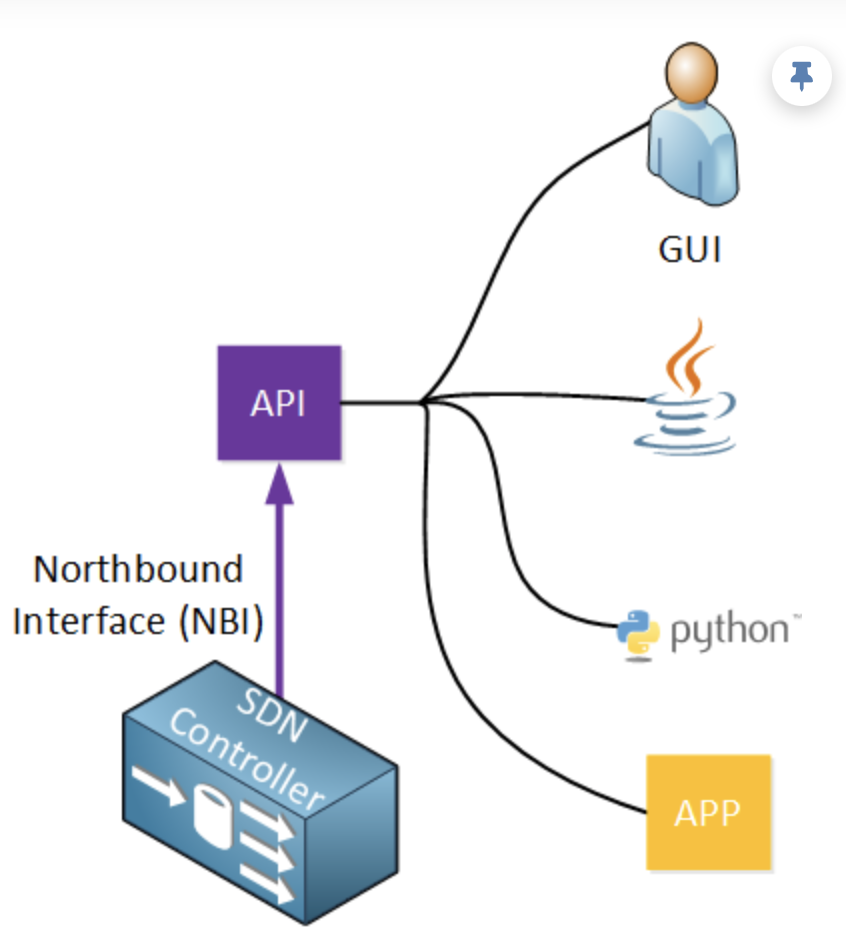
\includegraphics[scale=0.4]{images/sdn-16}
      %  \caption{A figure that is next to a certain explanation.}
      \end{figure}
    \end{column}
% Column 2
    \begin{column}{0.5\textwidth}
      \begin{itemize}[<+->]
      \item[\ding{219}] List information from all network devices in your network
      \item[\ding{219}] Show the status of all physical interfaces in the network
      \item [\ding{219}] Add a new VLAN on all your switches
      \item [\ding{219}] Show the topology of your entire network
      \item [\ding{219}] Automatically configure IP addresses, routing, and access-lists when a new virtual machine is created
    \end{itemize}
    \end{column}
  \end{columns}
\end{frame}

\begin{frame}
  \frametitle{Hands-on Demo Session}
  \begin{block}{Instructions at:}

    \url{https://github.com/kristjoc/org-mininet/}
  \end{block}
\end{frame}

\begin{frame}
  \frametitle{Mininet extensions}

  \begin{block}{\textbf{MaxiNet}} 
    MaxiNet extends the Mininet emulation environment to span the
    emulation across several physical machines in order to emulate
    very large software-defined networks.
  \end{block}

\end{frame}
%------------------------------------------------------------------------------%
\begin{frame}
  \frametitle{Mininet extensions}

  \begin{block}{MaxiNet}
  \end{block}
  \begin{block}{\textbf{DistriNet}}
    Distrinet is a distributed network emulator that provides a way to
    distribute Mininet over multiple hosts. Distrinet uses the same
    API as Mininet and it is fully compatible with Mininet programs.
  \end{block}
\end{frame}
%------------------------------------------------------------------------------%
\begin{frame}
  \frametitle{Mininet extensions}

  \begin{block}{MaxiNet}
  \end{block}
  \begin{block}{DistriNet}
  \end{block}
  \begin{block}{\textbf{Containernet}} 
    Containernet is a fork of the Mininet network emulator and allows
    to use Docker containers as hosts in emulated network topologies.
  \end{block}
\end{frame}
%------------------------------------------------------------------------------%
\begin{frame}[fragile]
  \frametitle{Containernet}

    \begin{block}{\textbf{Installation}}
    \rule{\textwidth}{0.5pt}
    \small
    \begin{minted}{bash}
      # First install Ansible:
      sudo apt-get install ansible
      # Then clone the repository:
      git clone https://github.com/containernet/containernet.git
      # Finally run the Ansible playbook to install required dependencies:
      sudo ansible-playbook -i "localhost," -c local \
                             containernet/ansible/install.yml
  \end{minted}
  \rule{\textwidth}{0.5pt}
\end{block}
\end{frame}
%------------------------------------------------------------------------------%
\begin{frame}[fragile]
  \frametitle{Containernet}

    \begin{block}{Installation}
    \end{block}
    \begin{block}{\textbf{Get started}}
    \rule{\textwidth}{0.5pt}
    \small
    \begin{minted}{bash}
      # First install Ansible:
      sudo apt-get install ansible
      # Then clone the repository:
      git clone https://github.com/containernet/containernet.git
      # Finally run the Ansible playbook to install required dependencies:
      sudo ansible-playbook -i "localhost," -c local \
                             containernet/ansible/install.yml
  \end{minted}
  \rule{\textwidth}{0.5pt}
\end{block}
\end{frame}
\begin{frame}[fragile]
  \frametitle{Containernet}

    \begin{block}{Installation}
    \end{block}
    \begin{block}{Get started}
    \end{block}
    \begin{block}{\textbf{Build container examples}}
    \rule{\textwidth}{0.5pt}
    \small
    \begin{minted}{bash}
      # Build containers
      sudo bash containernet/examples/example-containers/build.sh
  \end{minted}
  \rule{\textwidth}{0.5pt}
\end{block}
\end{frame}
\begin{frame}[fragile]
  \frametitle{Containernet}
    \begin{block}{Installation}
    \end{block}
    \begin{block}{Get started}
    \end{block}
    \begin{block}{Build container examples}
    \end{block}
    \begin{block}{\textbf{Run a basic example}}
    \rule{\textwidth}{0.5pt}
    \small
    \begin{minted}{bash}
      # Start an example topology
      sudo python3 examples/containernet_example.py
  \end{minted}
  \rule{\textwidth}{0.5pt}
\end{block}
\end{frame}


\begin{frame}[plain]
  \frametitle{In conclusion: Mininet can be your Swiss army knife for
    experimenting with networks and SDN.}

  \begin{textblock*}{7.9cm} (7cm,3.4cm) % {block width} (coords)
    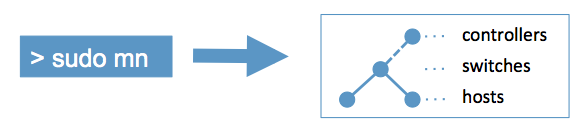
\includegraphics[width=7.9cm]{images/mininet.png}
    \captionsetup[figure]{justification=centering,font=footnotesize}
  \end{textblock*}

  \hspace{1cm}
  \large{\color{gray}Questions?}

  \begin{textblock*}{4cm} (1cm,7.55cm) % {block width} (coords)
    
\includegraphics[width=4cm]{images/uio-ifi.png}
  \end{textblock*}

  \begin{textblock*}{4cm} (11.36cm,7.55cm) % {block width} (coords)
    
\includegraphics[width=4cm]{images/ffi.png}
  \end{textblock*}

  \addtocounter{framenumber}{-1}
\end{frame}


\begin{frame}[plain]
  \frametitle{In conclusion: Mininet can be your Swiss army knife for
    experimenting with networks and SDN.}

  \begin{textblock*}{7.9cm} (7cm,3.4cm) % {block width} (coords)
    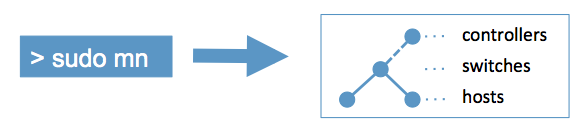
\includegraphics[width=7.9cm]{images/mininet.png}
    \captionsetup[figure]{justification=centering,font=footnotesize}
  \end{textblock*}

  \hspace{1cm}
  \large{Questions?}
  \begin{textblock*}{4cm} (1cm,7.55cm) % {block width} (coords)
    
\includegraphics[width=4cm]{images/uio-ifi.png}
  \end{textblock*}

  \begin{textblock*}{4cm} (11.36cm,7.55cm) % {block width} (coords)
    
\includegraphics[width=4cm]{images/ffi.png}
  \end{textblock*}

  \addtocounter{framenumber}{-1}
\end{frame}

\end{document}

%%% Local Variables:
%%% mode: latex
%%% TeX-master: t
%%% End:
